\chapter{Testing e Validazione}

\section{Strategia di Testing}
Testare un software per la migrazione dei dati è un aspetto fondamentale.
Data la sensibilità delle logiche del \textit{Data Dictionary} di Infor CloudSuite in ambienti Cloud Multitenant,
ogni anomalia nel record di inserimento avrebbe gravi conseguenze nel sistema di destinazione.

Inoltre, per il generatore dinamico di codice in Baan C, le procedure di prova
hanno incluso non solo l'importer dei dati, ma anche la correttezza sintattica e logica degli script
generati a runtime dalle DLL \texttt{txamgdll0012} e \texttt{txamgdll0013}.

\subsection{Unit Testing sui Moduli di Parsing}
I moduli di base (DLL quali \texttt{txamgdll0011}) per l'estrazione e la gestione dei metadata (\textit{metadata management})
degli Infor Exchange sono stati testati su porzioni specifiche di file.

Verificando ogni singola colonna (\texttt{txamg1111}), la validazione include il corretto casting di tipi enumerati,
decimali a virgola mobile e codifiche caratteri ASCII, simulando una diversità di input.
Durante questa fase si vede come i cambi di versione della destinazioni non alterino le librerie costruite se le posizioni di inizio (\texttt{stpn}) e la lunghezza (\texttt{leng}) vengono mantenute.

\subsection{Test del Flusso di Migrazione}
L'integrazione end-to-end è validata eseguendo flussi di test governati dalle logiche di batch (\texttt{txamg2100}
e \texttt{txamg3200}). Durante questi test, il sistema genera gli script di elaborazione e li sottopone al compilatore interno \texttt{bic\_compiler}.
Se la generazione avviene correttamente, lo script compilato viene agganciato al batch e lanciato.

\begin{figure}[H]
	\centering
	\tikzset{
		io_small/.style={trapezium, trapezium left angle=70, trapezium right angle=110, minimum width=2.2cm, minimum height=0.8cm, text centered, draw=black, fill=blue!30, font=\footnotesize},
		proc_small/.style={rectangle, minimum width=2.5cm, minimum height=0.8cm, text centered, draw=black, fill=orange!25, font=\footnotesize},
		dec_small/.style={diamond, aspect=1.5, minimum width=2.5cm, minimum height=0.8cm, text centered, draw=black, fill=green!25, font=\footnotesize},
		arrow/.style={thick,->,>=stealth}
	}
	\resizebox{\textwidth}{!}{
		\begin{tikzpicture}[node distance=1cm and 1.2cm]
			\node (raw) [io_small] {File Originario};
			\node (read) [proc_small, right=of raw] {Lettura ed Estrazione (rere)};
			\node (dec2) [dec_small, right=of read] {Validazione record};
			\node (proc) [proc_small, right=of dec2] {Record Elaborato (repr)};
			\node (disc) [proc_small, below=of dec2, yshift=-0.3cm] {Scarto Record (reer)};
			\draw [arrow] (raw) -- (read);
			\draw [arrow] (read) -- (dec2);
			\draw [arrow] (dec2) -- node[midway, below, font=\scriptsize] {Superata} (proc);
			\draw [arrow] (dec2) -- node[midway, left, font=\scriptsize] {Non Superata} (disc);
			\draw [arrow, dashed] (read.north west) .. controls +(0.4,0.8) and +(-0.4,0.8) .. (read.north east)
			node[midway, above, font=\scriptsize] {Total Volume};
		\end{tikzpicture}
	}
	\caption{Rappresentazione logica del matching numerico di integrità}
	\label{fig:matching_logico_testing}
\end{figure}

Un aspetto rilevante del testing d'integrazione riguarda la misurazione dei tempi di run.
Durante le simulazioni, con recordset di piccole (circa $1.000$ inserimenti) e medie dimensioni (sino a $50.000$ righe),
sono state effettuate delle misurazioni sulle latenze introdotte dal caricamento cloud e dai vincoli di referenzialità.
In parallelo, per assicurare le prestazioni e le procedure di rollback, qualora ci siano rallentamenti o blocchi a livello di rete,
il motore transazionale LN è stato istruito affinché le commit avvengano a blocchi così come stabilito del numero di record.
Questo è stato confermato dai casi d'uso in cui il server restituisce messaggi di \textit{Timeout}.

\begin{figure}[H]
	\centering
	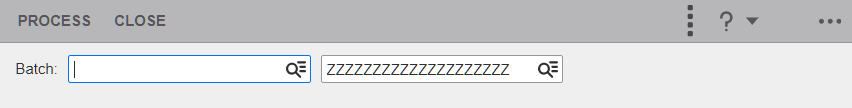
\includegraphics[width=0.8\textwidth]{Immagini/Sessioni/ExecuteBatchRuns_txamg3200m000}
	\caption{Sessione di Esecuzione Batch (txamg3200m000)}
	\label{fig:sessione_esecuzione_batch}
\end{figure}

I \textit{Runs Errors} offrono un riscontro immediato di blocchi logici o semantici.
Sono stati eseguiti scenari in cui la validazione è forzata per respingere record privi di riferimenti chiave,
verificando che la linea errata fosse elaborata senza però interromperne il caricamento dell'intero \textit{Run}.

\begin{figure}[H]
	\centering
	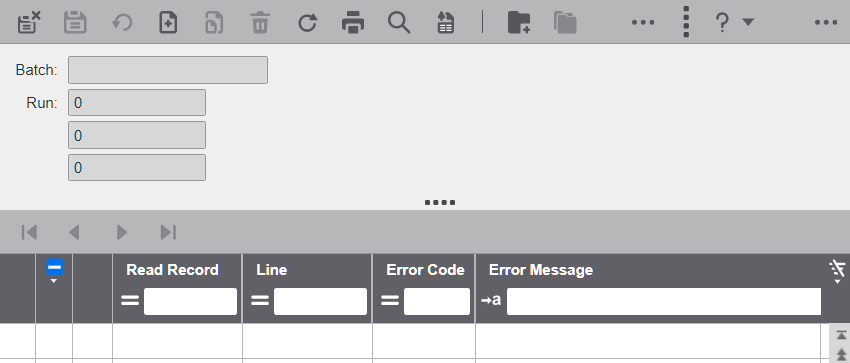
\includegraphics[width=0.8\textwidth]{Immagini/Sessioni/RunsErrors_txamg3503m000}
	\caption{Dettaglio degli errori di migrazione (txamg3503m000)}
	\label{fig:dettaglio_errori_migrazione}
\end{figure}

Gli errori segnalati sono dettagliati all'interno della tabella \texttt{txamg303}, le cui colonne principali permettono
di investigare quale linea e record sia fallito:
\begin{itemize}
    \item \texttt{runs}: Identificativo del Run
    \item \texttt{rere}: Riga di lettura (\textit{Read Record})
    \item \texttt{line}: Riga testuale all'interno del file sorgente
    \item \texttt{errc}: Codice specifico dell'errore (\textit{Error Code})
    \item \texttt{errm}: Descrizione del problema riscontrato dal DAL (\textit{Error Message})
\end{itemize}

Oltre ai controlli manuali, questo tracciamento funge da base per le strategie di \textit{retry} o per
le \textit{sanity check} del dato prima della re-immissione: individuando la tipologia di errore, il consulente o l'operatore
può decidere se modificarne il mapping, apportare modifiche sul file d'origine o creare estensioni
specifiche ai moduli generati dal tool.

\section{Verifica dell'Integrità dei Dati}
\subsection{Matching tra Dati Sorgente (Legacy) e Destinazione (Cloud)}
Ogni file migrato viene tracciato sulle tabelle atte al monitoraggio (\texttt{txamg301}, \texttt{txamg302}). Il \textit{matching}
prevede che vengano comparati il numero dei record letti, processati ed eventualmente respinti rispetto all'origine.
Questo consente di ottenere la garanzia del risultato atteso, in quanto una discrepanza nel numero di dati letti e scritti,
segnalerebbe un errore evidente.

Nello specifico la tabella \texttt{txamg301} incapsula le metriche di base del processo:
\begin{longtable}{@{} l p{4cm} p{7cm} @{}}
    \toprule
    \textbf{Campo} & \textbf{Nome} & \textbf{Descrizione} \\
    \midrule
    \endfirsthead
    \toprule
    \textbf{Campo} & \textbf{Nome} & \textbf{Descrizione} \\
    \midrule
    \endhead
    \midrule
    \multicolumn{3}{r}{{Continua nella pagina successiva}} \\
    \bottomrule
    \endfoot
    \bottomrule
    \caption{Struttura dei conteggi per l'affidabilità (txamg301)}
    \endlastfoot
    \texttt{rere} & Records Read & Il volume totale delle istruzioni e record processati dal tool \\
    \texttt{repr} & Record Processed & Quanti dei record immessi hanno dato esito positivo dopo tutti i trigger \\
    \texttt{reer} & Records Discarded & Numero di istanze rifiutate o bloccate dal check del DB \\
\end{longtable}

I report prodotti (tramite moduli ad hoc come \texttt{txamgdll0011} per il log d'errore) forniscono la garanzia
numerica dell'operazione, permettendo al team di validazione di avere stime certe prima dell'import su CloudSuite finale.

Questo approccio garantisce che le disconnessioni di rete o i blocchi temporanei non lascino i dati in uno stato di
incertezza.
Il tool si comporta in maniera deterministica e produce riscontri sempre validati rispetto al totale.

\begin{figure}[H]
	\centering
	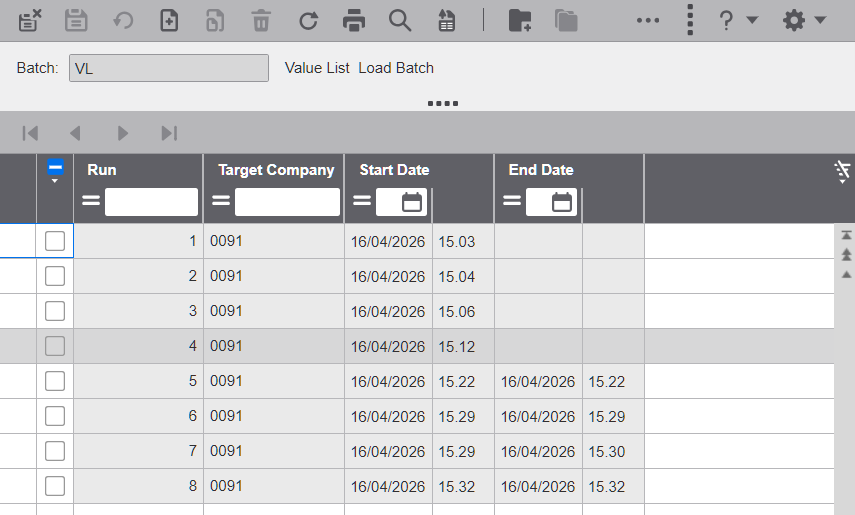
\includegraphics[width=0.8\textwidth]{Immagini/Sessioni/RunsByBatch_txamg3500m000}
	\caption{Storico e validazione delle esecuzioni (txamg3500m000)}
	\label{fig:storico_validazione_runs}
\end{figure}
